\documentclass[12pt,a4paper]{article}
\usepackage[margin=1in]{geometry}
\usepackage{parskip}
\usepackage{microtype}
\usepackage{booktabs}
\usepackage{graphicx}
\usepackage{amsmath,amssymb}
\usepackage[most]{tcolorbox}

\title{A basis for the difference curve\\[0.4em]\large and whether its coefficients are integers}
\author{Robin Langer}
\date{}

\begin{document}
\maketitle
\vspace{-1.5em}

\section{The curve}

Let $L(n)$ be the period of the continued fraction of $\sqrt n$ and $t = L(n)/\sqrt n$. Fitting a Weibull to the values of $t$ for every non-square $n < M$ leaves a residual, and the cleanest form of it is cumulative:
\[
  D(t) \;=\; F_{\text{empirical}}(t) \;-\; F_{\text{Weibull}}(t) .
\]
It is pinned at $0$ at both ends, rises to $+0.019$ near $t = 0.29$, crosses zero near $0.64$, dips to about $-0.007$ through the middle, and recovers. Its largest excursion is the Kolmogorov--Smirnov statistic.

This document asks what function it is.

\section{How well the curve is known}

Before fitting anything, the accuracy of the target. $D$ still moves with $M$: between $M = 600{,}000$ and $M = 10^6$,
\[
  \sup|D_{10^6} - D_{6\times10^5}| = 0.000733,
  \qquad
  \mathrm{rms} = 0.000257 ,
\]
against $\mathrm{rms}(D) = 0.006733$. So the curve is known to about four percent of its own size.

\begin{tcolorbox}[colback=red!5, colframe=red!45!black, arc=2mm]
\textbf{Any fit reaching an rms residual below $0.000257$ is fitting the drift and not the shape.} This bounds the whole exercise, and it is drawn on every figure below. Comparisons between bases are meaningful in the four- and six-term columns, marginal at eight, and meaningless at ten.
\end{tcolorbox}

\section{Three families that are the same family}

\begin{center}
\begin{tabular}{lrrrr}
\toprule
 & 4 terms & 6 & 8 & 10 \\
\midrule
monomials $1,x,x^2,\ldots$ & $0.005088$ & $0.002612$ & $0.001086$ & $0.000918$ \\
Legendre, no weight        & $0.005088$ & $0.002612$ & $0.001086$ & $0.000918$ \\
Chebyshev, no weight       & $0.005088$ & $0.002612$ & $0.001086$ & $0.000918$ \\
\bottomrule
\end{tabular}
\end{center}

Identical to six decimals, at every term count, and this is not a numerical accident. Polynomials of degree less than $n$ span the same $n$-dimensional space whichever family they are drawn from, so least squares finds the same element of that space. Changing from $x^n$ to Chebyshev buys conditioning --- the monomial design matrix is badly behaved for large $n$ --- and changes the answer not at all.

The consequence is worth stating plainly: \emph{an unweighted orthogonal expansion is a monomial fit in costume}. Any genuine gain comes from a weight function, not from the polynomials.

\section{The weight does the work}

\begin{center}
\begin{tabular}{lrrrr}
\toprule
 & 4 terms & 6 & 8 & 10 \\
\midrule
unweighted polynomials                       & $0.005088$ & $0.002612$ & $0.001086$ & $0.000918$ \\
Hermite $\times\, e^{-u^2/2}$, $u=(t-m)/s$   & $0.002942$ & $\mathbf{0.000658}$ & $0.000657$ & $0.000522$ \\
Laguerre $\times\, e^{-bt}$                  & $0.001923$ & $0.000848$ & $0.000665$ & $0.000281$ \\
generalised Laguerre, $\alpha=1$             & $0.001741$ & $0.000970$ & $\mathbf{0.000510}$ & $0.000440$ \\
generalised Laguerre, $\alpha=0.149$         & $0.001793$ & $0.000819$ & $0.000526$ & $0.000205$ \\
rational Chebyshev on $[0,\infty)$, $\beta=0.855$ & $0.002036$ & $0.000705$ & $0.000613$ & $0.000439$ \\
exponential CDFs on a ladder of scales       & $\mathbf{0.001332}$ & $0.000821$ & $0.000665$ & $0.000503$ \\
Bernstein after the probability transform    & $0.003925$ & $0.001719$ & $0.001247$ & $0.000999$ \\
shifted Legendre after the transform         & $0.001939$ & $0.001310$ & $0.001072$ & $0.000898$ \\
sine series after the transform              & $0.003176$ & $0.002343$ & $0.001961$ & $0.001713$ \\
\bottomrule
\end{tabular}
\end{center}

\begin{center}
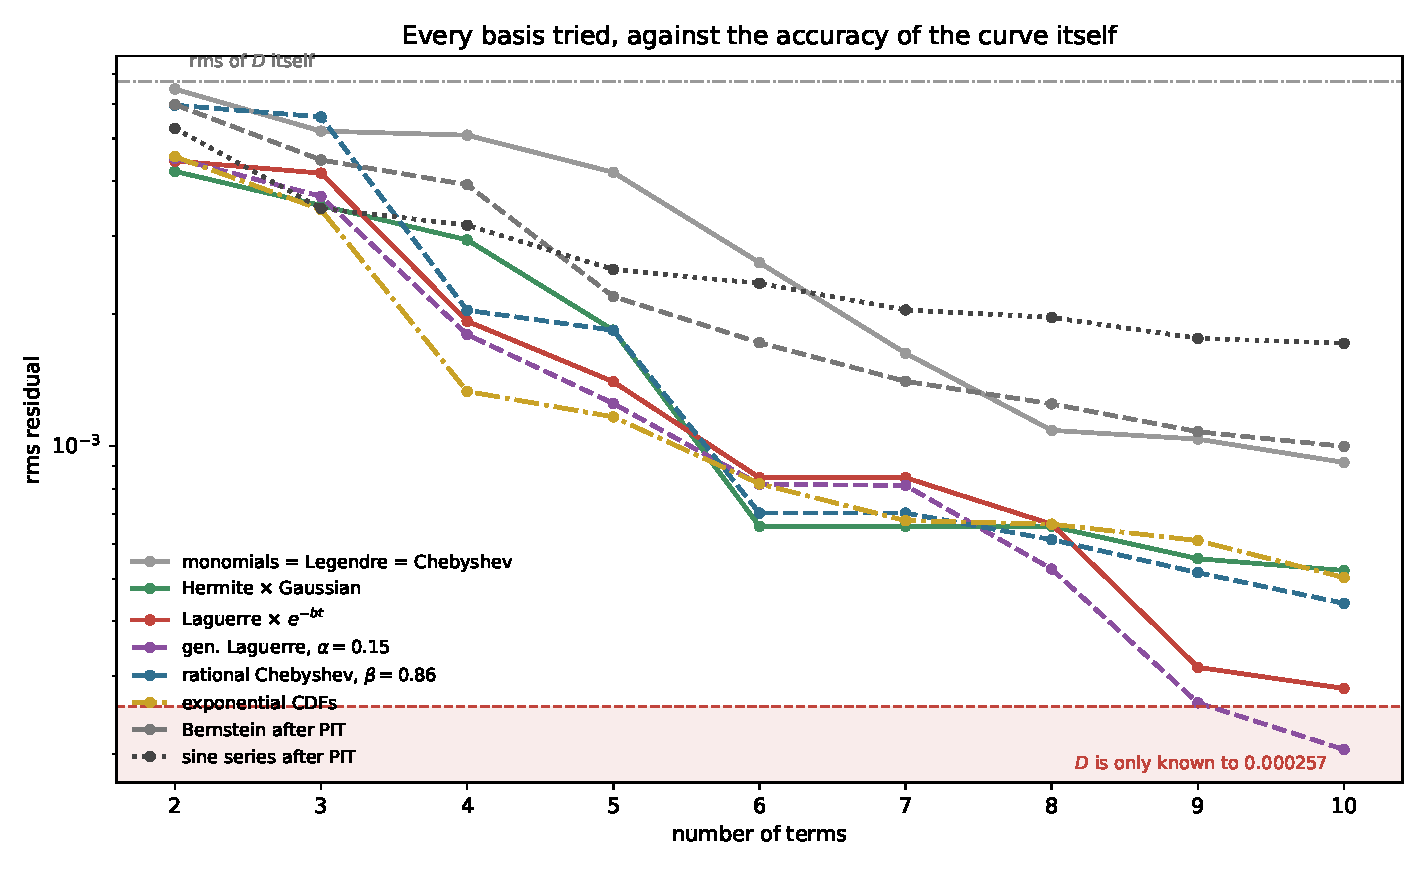
\includegraphics[width=0.92\textwidth]{bases-figure.pdf}
\end{center}

Weighting by $e^{-bt}$ or $e^{-u^2/2}$ improves the six-term fit by a factor of three to four, because the envelope already carries the exponential decay of $D$ and leaves the polynomial to supply only shape. The unweighted families must spend terms manufacturing the decay before they can begin.

Between the two classical choices, Hermite is better at six terms and Laguerre at ten, but Laguerre is the principled one: it is orthogonal on $[0,\infty)$, which is where $D$ lives, whereas Hermite is borrowed from the whole line by a shift. Note the flat step in the Hermite row from six terms to eight, $0.000658$ to $0.000657$: the seventh term contributes nothing, which is a parity signature of the Gram--Charlier form.

Two further remarks from the table. Fitting the exponent of the generalised Laguerre weight $t^\alpha e^{-bt}$ gives $\alpha = 0.149$, not $1$ --- so $D$ approaches the origin far more weakly than linearly, which is the sharp discreteness dip, $t$ being unable to fall below $1/\sqrt n$. And rational Chebyshev, which maps $[0,\infty)$ to $[-1,1]$ by $x = (t-\beta)/(t+\beta)$ and assumes \emph{no} decay rate at all, is second best at six terms. That is mild evidence that the true tail of $D$ is not exponential.

\section{The basis that should have won}

The sine series is last, and it is the one with the strongest theoretical claim.

After the probability integral transform $u = F_{\text{Weibull}}(t)$, the empirical process converges to a Brownian bridge on $[0,1]$. The Karhunen--Lo\`eve basis of that bridge is exactly
\[
  \sqrt{2}\,\sin(k\pi u), \qquad \text{eigenvalues } \frac{1}{k^2\pi^2},
\]
which is the optimal basis for representing its sample paths, and is what stands behind the Cram\'er--von Mises and Anderson--Darling statistics.

It fails here, and the failure is the point. That basis is efficient for \emph{random} departures from the fitted law. Ours is not random --- it is a fixed systematic shape, with no reason to be sparse in the eigenbasis of the noise. The poor showing of the bridge basis is one more demonstration, from a new direction, that the residual is not sampling error.

\section{Are the coefficients integers?}

No, and the question as posed has no answer.

Coefficients carry the arbitrary overall scale of $D$, so only ratios between them could mean anything. But the ratios are not determined by the data: the Laguerre expansion has a free scale $b$, fixed here by least squares, and the fit is flat in it.

\begin{center}
\begin{tabular}{rrrrl}
\toprule
$b$ & rms & $c_1/c_3$ & nearest simple & gap \\
\midrule
$4.400$ & $0.001089$ & $0.6262$ & $5/8$  & $0.0012$ \\
$4.800$ & $0.001004$ & $0.3944$ & $2/5$  & $0.0056$ \\
$5.200$ & $0.000905$ & $0.3056$ & $3/10$ & $0.0056$ \\
$5.657$ & $0.000848$ & $0.2523$ & $1/4$  & $0.0023$ \\
$6.000$ & $0.000886$ & $0.2259$ & $2/9$  & $0.0037$ \\
$6.500$ & $0.001063$ & $0.1974$ & $1/5$  & $0.0026$ \\
$7.000$ & $0.001320$ & $0.1749$ & $2/11$ & $0.0070$ \\
\bottomrule
\end{tabular}
\end{center}

Every value of $b$ from $4.56$ to $6.49$ fits within $25\%$ of the best. Over that range $c_1/c_3$ sweeps continuously from $0.499$ to $0.198$, crossing \emph{fifteen} distinct rationals of denominator at most twelve. And at every row of the table the nearest simple fraction is within $0.007$, which is exactly what one should expect: rationals of denominator at most twelve sit about $0.005$ apart in this range, so any real number is that close to one.

\begin{center}
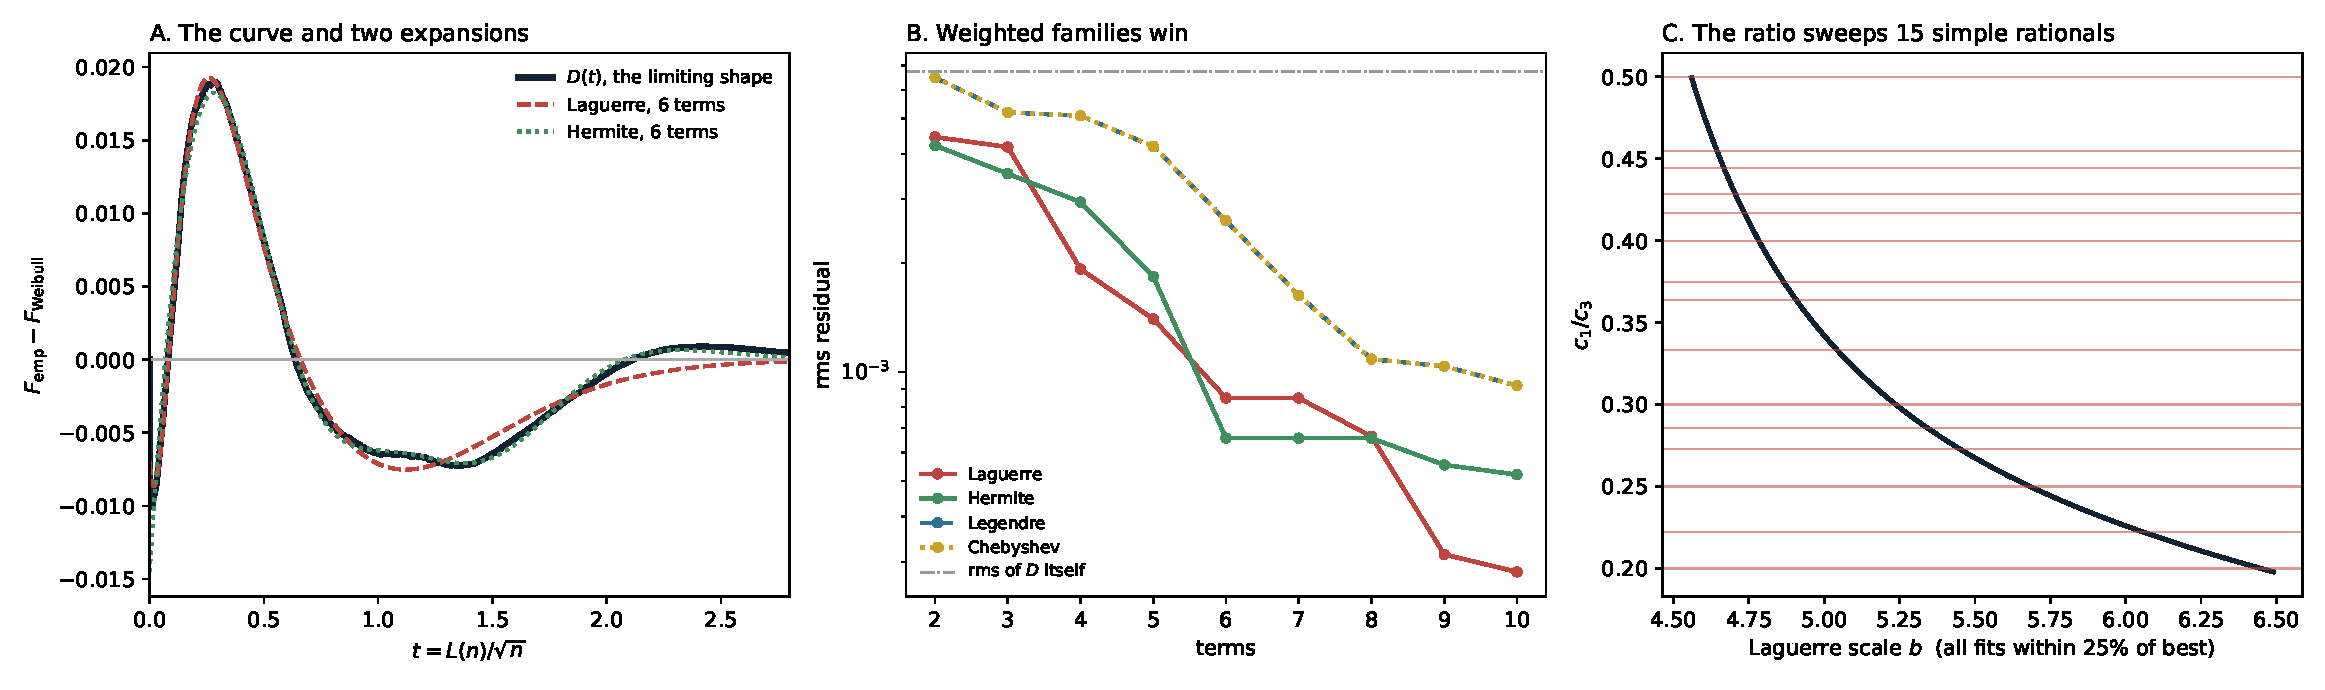
\includegraphics[width=\textwidth]{orthogonal.pdf}
\end{center}

An earlier pass flagged four ratios as promising, on the grounds that they were stable to a thousandth between $M = 6\times10^5$ and $10^6$. Stability under more \emph{data} looks like a test and is not one here, because the free parameter was never the data. Hold the data fixed, move $b$ within its tolerance, and the same ratio visits fifteen rationals in turn.

\begin{tcolorbox}[colback=blue!6, colframe=blue!45!black, arc=2mm]
An integrality claim requires the scale to be fixed by something outside the fit --- a decay rate that can be derived, or a normalisation the problem itself supplies. Tuned by least squares, ``is this coefficient rational?'' has no truth value.
\end{tcolorbox}

\section{What to use}

For accuracy at a small number of terms, generalised Laguerre with the weight $t^{0.149}e^{-bt}$, or rational Chebyshev if one would rather not assume the tail.

For meaning, none of them. The basis of exponential distribution functions on a ladder of scales is best at four terms and is the only one whose coefficients say anything outside the fit: they are weights on scales, and the mixture over scales is the class number. A two-component version of it cuts the Kolmogorov--Smirnov distance from $14.0$ to $3.4$ times its critical value. Every polynomial basis in this document produces numbers that are true of the fit and of nothing else.

\end{document}
